\documentclass{article}
\usepackage{float, hyperref}
\usepackage[margin=1in]{geometry}
\usepackage{graphicx}
\usepackage{hyperref}
\usepackage{caption}
\usepackage{pgffor}

\title{Replication Script to JSS Submission}
\usepackage{Sweave}
\begin{document}


\author{Lindsay Rutter, Susan VanderPlas, Dianne Cook, Michelle A. Graham}
\date{\today}
\maketitle
\Sconcordance{concordance:replicationScript.tex:replicationScript.Rnw:%
1 3 1 1 0 14 1 1 2 1 0 3 1 11 0 1 2 2 1 1 2 1 0 1 1 5 0 1 1 6 0 1 2 3 1}


%%%%%%%%%%%%%%%
%% Section 2 %%
%%%%%%%%%%%%%%%
\section*{2. Available software}

The two figures in this section of the paper (Figure 1 and 2) were not produced using source code from our ggenealogy package. Instead, they were produced from external software for demonstration purposes.

%%%%%%%%%%%%%%%
%% Section 3 %%
%%%%%%%%%%%%%%%
\section*{3. Example datasets}

First, we can load and examine the structure of the example soybean genealogy dataset (called sbGeneal):

\begin{Schunk}
\begin{Sinput}
> rm(list=)
> library("devtools")
> load_all("ggenealogy")
> library("ggenealogy")
> data("sbGeneal")
> str(sbGeneal)
\end{Sinput}
\begin{Soutput}
'data.frame':	390 obs. of  5 variables:
 $ child       : chr  "5601T" "Adams" "A.K." "A.K. (Harrow)" ...
 $ year        : num  1981 1948 1910 1912 1968 ...
 $ yield       : int  NA 2734 NA 2665 NA 2981 2887 2817 NA NA ...
 $ year.imputed: logi  TRUE FALSE TRUE FALSE FALSE FALSE ...
 $ parent      : chr  "Hutcheson" "Dunfield" NA "A.K." ...
\end{Soutput}
\end{Schunk}

After that, we can load and examine the structure of the example academic statistician genealogy dataset (called statGeneal):

\begin{Schunk}
\begin{Sinput}
> data("statGeneal")
> dim(statGeneal)
\end{Sinput}
\begin{Soutput}
[1] 8165    6
\end{Soutput}
\begin{Sinput}
> colnames(statGeneal)
\end{Sinput}
\begin{Soutput}
[1] "child"   "parent"  "year"    "country" "school"  "thesis" 
\end{Soutput}
\end{Schunk}

%%%%%%%%%%%%%%%
%% Section 5 %%
%%%%%%%%%%%%%%%
\section*{5. Generating a graphical object}

We can convert our example soybean genealogy dataset (called sbGeneal) into an igraph object:

\begin{Schunk}
\begin{Sinput}
> sbIG <- dfToIG(sbGeneal)
> sbIG
\end{Sinput}
\begin{Soutput}
IGRAPH UNW- 230 340 -- 
+ attr: name (v/c), weight (e/n)
+ edges (vertex names):
 [1] 5601T    --Hutcheson        Adams    --Dunfield        
 [3] A.K.     --A.K. (Harrow)    Altona   --Flambeau        
 [5] Amcor    --Amsoy 71         Adams    --Amsoy           
 [7] Amsoy 71 --C1253            Anderson --Lincoln         
 [9] Bay      --York             Bedford  --Forrest         
[11] Beeson   --Kent             Blackhawk--Richland        
[13] Bonus    --C1266R           Bradley  --J74-39          
[15] Bragg    --Jackson          Bragg    --Bragg x D60-7965
+ ... omitted several edges
\end{Soutput}
\end{Schunk}

Now that we have an igraph object, we can obtain basic summary statistics about it:

\begin{Schunk}
\begin{Sinput}
> getBasicStatistics(sbIG)
\end{Sinput}
\begin{Soutput}
$isConnected
[1] FALSE

$numComponents
[1] 11

$avePathLength
[1] 5.333746

$graphDiameter
[1] 13

$numNodes
[1] 230

$numEdges
[1] 340

$logN
[1] 5.438079
\end{Soutput}
\end{Schunk}

%%%%%%%%%%%%%%%
%% Section 6 %%
%%%%%%%%%%%%%%%
\section*{6. Plotting a shortest path}

At this point, we can determine the shortest path of parent-child relationships between two labels of interest ("Tokyo" and "Narow").

\begin{Schunk}
\begin{Sinput}
> pathTN <- getPath("Tokyo", "Narow", sbIG, sbGeneal)
> pathTN
\end{Sinput}
\begin{Soutput}
$pathVertices
[1] "Tokyo"    "Volstate" "Jackson"  "R66-873"  "Narow"   

$yearVertices
[1] "1907"   "1942"   "1954.5" "1971.5" "1985"  
\end{Soutput}
\end{Schunk}

The returned path can then be plotted.

\begin{Schunk}
\begin{Sinput}
> plotPath(pathTN)
\end{Sinput}
\end{Schunk}

\begin{figure}[H]
\centering
\begin{Schunk}
\begin{Sinput}
> plotPath(pathTN)
\end{Sinput}
\end{Schunk}
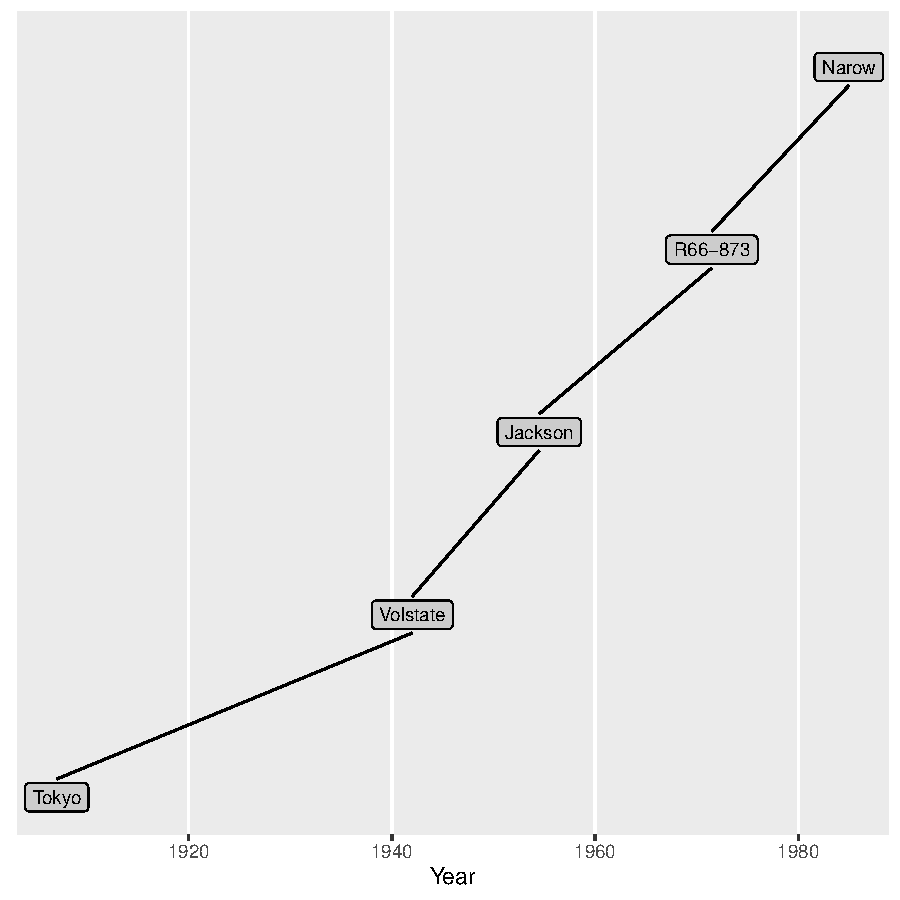
\includegraphics{replicationScript-008}
\end{figure}

We can do the same for a different pair of two labels of interest ("Bedford" and "Zane"). First, we can determine the years these two labels were identified.

\begin{Schunk}
\begin{Sinput}
> getYear("Bedford", sbGeneal)
\end{Sinput}
\begin{Soutput}
[1] 1978
\end{Soutput}
\begin{Sinput}
> getYear("Zane", sbGeneal)
\end{Sinput}
\begin{Soutput}
[1] 1985
\end{Soutput}
\end{Schunk}

Next, we can determine the shortest path of parent-child relationships between these two labels of interest and plot it.

\begin{Schunk}
\begin{Sinput}
> pathBZ <- getPath("Bedford", "Zane", sbIG, sbGeneal)
> plotPath(pathBZ, fontFace = 2)
\end{Sinput}
\end{Schunk}

%%%%%%%%%%%%%%%
%% Section 7 %%
%%%%%%%%%%%%%%%
\section*{7. Superimposing shortest path on tree}

In the previous section, we obtained the shortest path between the the pair of labels "Tokyo" and "Narow" and saved it as a variable pathTN. Here, we can plot that path superimposed over all labels in the example soybean genealogy dataset.

\begin{Schunk}
\begin{Sinput}
> plotPathOnAll(pathTN, sbGeneal, sbIG, binVector = 1:3, pathEdgeCol = "red", nodeSize = 2.5, pathNodeSize = 4) + ggplot2::theme(axis.text = ggplot2::element_text(size = 12), axis.title = ggplot2::element_text(size = 12))
\end{Sinput}
\end{Schunk}

We can repeat this process, only now instead of setting the binVector variable to 1:3 (as we did earlier), we can set it to 1:6.

\begin{Schunk}
\begin{Sinput}
> plotPathOnAll(pathTN, sbGeneal, sbIG, binVector = 1:6, pathEdgeCol = "seagreen2", nodeSize = 1, pathNodeSize = 3)
\end{Sinput}
\end{Schunk}

%%%%%%%%%%%%%%%
%% Section 8 %%
%%%%%%%%%%%%%%%
\section*{8. Plotting ancestors and descendants by generation}

As is explained in the article, only the top part of Figure 6 (the figure from this section) is produced by ggenealogy code. In contrast, the bottom part of Figure 6 was produced by tools outside of ggenealogy for didactic purposes. Below, we recreate the top part of Figure 6, which was to generate a plot of the ancestors and descendants of the label Lee.

\begin{Schunk}
\begin{Sinput}
> plotAncDes("Lee", sbGeneal, mAnc = 6, mDes = 6, vCol = "blue")
\end{Sinput}
\end{Schunk}

%%%%%%%%%%%%%%%
%% Section 9 %%
%%%%%%%%%%%%%%%
\section*{9. Plotting distance matrix}

We can plot the distance matrix for a set of 10 varieties.

\begin{Schunk}
\begin{Sinput}
> varieties <- c("Brim", "Bedford", "Calland", "Dillon", "Hood", "Narow", "Pella", "Tokyo", "Young", "Zane")
> plotDegMatrix(varieties, sbIG, sbGeneal, "Variety", "Variety", "Degree") + ggplot2::scale_fill_continuous(low = "white", high = "darkgreen") + ggplot2::theme(legend.title = ggplot2::element_text(size = 15), legend.text = ggplot2::element_text(size = 15))
\end{Sinput}
\end{Schunk}

%%%%%%%%%%%%%%%%
%% Section 10 %%
%%%%%%%%%%%%%%%%
\section*{10. Academic genealogy of statisticians}

We can now explore some of the plotting functions in ggenealogy, only now with the academic statistican genealogy dataset. This second example dataset is much larger than the first example dataset of soybean genealogy. For example purposes, we would like to view the ancestor and descendant plot for the individual who has the largest number of descendants. To identify the name of this individual, we run the following code:

\begin{Schunk}
\begin{Sinput}
> library("dplyr")
> indVec <- getNodes(statGeneal)
> indVec <- indVec[which(indVec != "", )]
> dFunc <- function(var) nrow(getDescendants(var, statGeneal, gen = 100))
> numDesc <- sapply(indVec, dFunc)
> table(numDesc)
\end{Sinput}
\begin{Soutput}
numDesc
   0    1    2    3    4    5    6    7    8    9   10   11   12   13   14   15 
6251  322  145   88   58   36   31   22   23   14   17   13   14   10    9    6 
  16   17   18   19   20   21   22   23   24   25   26   27   29   30   34   37 
   4    3    2    5    7    4    3    3    2    2    6    1    1    3    2    1 
  38   40   41   44   45   48   49   60   61   75   77   84  159 
   1    1    1    1    1    1    2    1    1    1    1    1    1 
\end{Soutput}
\begin{Sinput}
> which(numDesc == 159)
\end{Sinput}
\begin{Soutput}
David Cox 
     1980 
\end{Soutput}
\end{Schunk}

We see the individual with the largest number of descendants is Sir David Cox, who has 159 descendants. Now, we can plot the "ancestors" and "descendants" of Sir David Cox.

\begin{Schunk}
\begin{Sinput}
> plotAncDes("David Cox", statGeneal, mAnc = 6, mDes = 6, vCol = "blue")
\end{Sinput}
\end{Schunk}

It seems that of the 42 "children" of Sir David Cox, the one who went on to have the largest number of "children" of his own was Peter Bloomfield. We can verify below that Peter Bloomfield had 26 "children" and 49 "descendants".

\begin{Schunk}
\begin{Sinput}
> length(getChild("Peter Bloomfield", statGeneal))
\end{Sinput}
\begin{Soutput}
[1] 26
\end{Soutput}
\begin{Sinput}
> nrow(getDescendants("Peter Bloomfield", statGeneal, gen = 100))
\end{Sinput}
\begin{Soutput}
[1] 49
\end{Soutput}
\end{Schunk}

It would be of interest now to examine the shortest path between Sir David Cox and one of his newest "descendants" Petra Buzkova. To do so, we first need to obtain the corresponding igraph object of the example academic statistican genealogy dataset.

\begin{Schunk}
\begin{Sinput}
> statIG <- dfToIG(statGeneal)
\end{Sinput}
\end{Schunk}

After doing so, we can now determine the shortest path between Sir David Cox and Petra Buzkova, and plot it.

\begin{Schunk}
\begin{Sinput}
> pathCB <- getPath("David Cox", "Petra Buzkova", statIG, statGeneal, isDirected = FALSE)
> plotPath(pathCB, fontFace = 4) + ggplot2::theme(axis.text = ggplot2::element_text(size = 10), axis.title = ggplot2::element_text(size = 10)) + ggplot2::scale_x_continuous(expand = c(.1, .2))
\end{Sinput}
\end{Schunk}

We can now superimpose this shortest path between Sir David Cox and Petra Buzkova across the entire genealogical structure.

\begin{Schunk}
\begin{Sinput}
> plotPathOnAll(pathCB, statGeneal, statIG, binVector = 1:200) + ggplot2::theme(axis.text = ggplot2::element_text(size = 8), axis.title = ggplot2::element_text(size = 8)) + ggplot2::scale_x_continuous(expand = c(.1, .2))
\end{Sinput}
\end{Schunk}

We notice, however, that we cannot read the text of the nodes on the path of interest. To solve this problem, we can create the same plot, only now specifying that any nodes that are not on our path of interest are deemphasized with smaller text.

\begin{Schunk}
\begin{Sinput}
> plotPathOnAll(pathCB, statGeneal, statIG, binVector = 1:200, nodeSize = .5, pathNodeSize = 2.5, nodeCol = "darkgray", edgeCol = "lightgray") + ggplot2::theme(axis.text = ggplot2::element_text(size = 8), axis.title = ggplot2::element_text(size = 8)) + ggplot2::scale_x_continuous(expand = c(.1, .2))
\end{Sinput}
\end{Schunk}

Even though we can now read the text labels on the path of interest, we lost the ability to read labels that are not on our path of interest. At this point, we can keep the best of both worlds: We can create a plot that demphasizes the nodes that are not on the path of interest by assigning them small text font size, but incoroporate an interactive function so that we can hover over these non-path nodes if we wish to obtain their label information. This is the plot we used and interacted with to create the video embedded in Figure 12.

\begin{Schunk}
\begin{Sinput}
> plotPathOnAll(pathCB, statGeneal, statIG, binVector = 1:200, nodeSize = .5, pathNodeSize = 2.5, nodeCol = "darkgray", edgeCol = "lightgray", animate = TRUE)
\end{Sinput}
\end{Schunk}

\end{document}
